\large
\begin{multicols}{2}
	\begin{itemize}
		\item Revolução neolítica
		\item $\sim$ 10.000 a.C ou antes
		\item princípio da tecelagem
		\normalsize
		\begin{itemize}
		\item teias de aranha
		\item ninhos de pássaro
		\item pequenos galhos
		\item barreiras
		\item escudos
		\item cestas
		\item habitações
		\end{itemize}
		 \item Tecidos
	
	\end{itemize}
	
	\vfill\null
\columnbreak

\vspace*{-15mm}
\begin{center}
	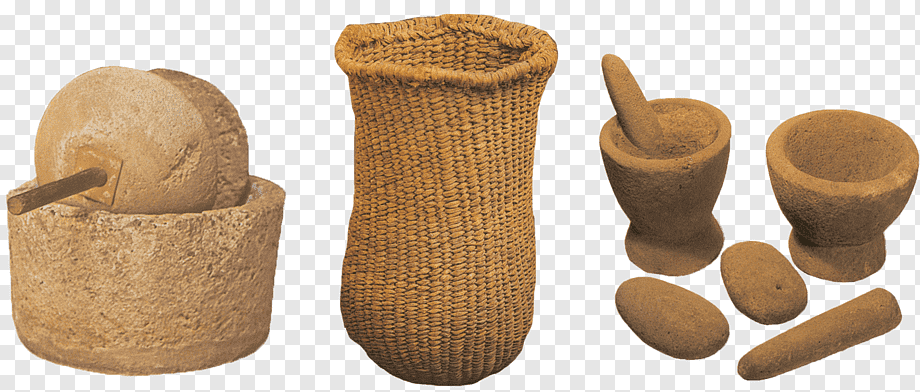
\includegraphics[width=.8\linewidth]{./IMG/png-transparent-neolithic-revolution-paleolithic-prehistory-mesolithic-homens-textile-pottery-revolution.png}
\end{center}

\begin{center}
	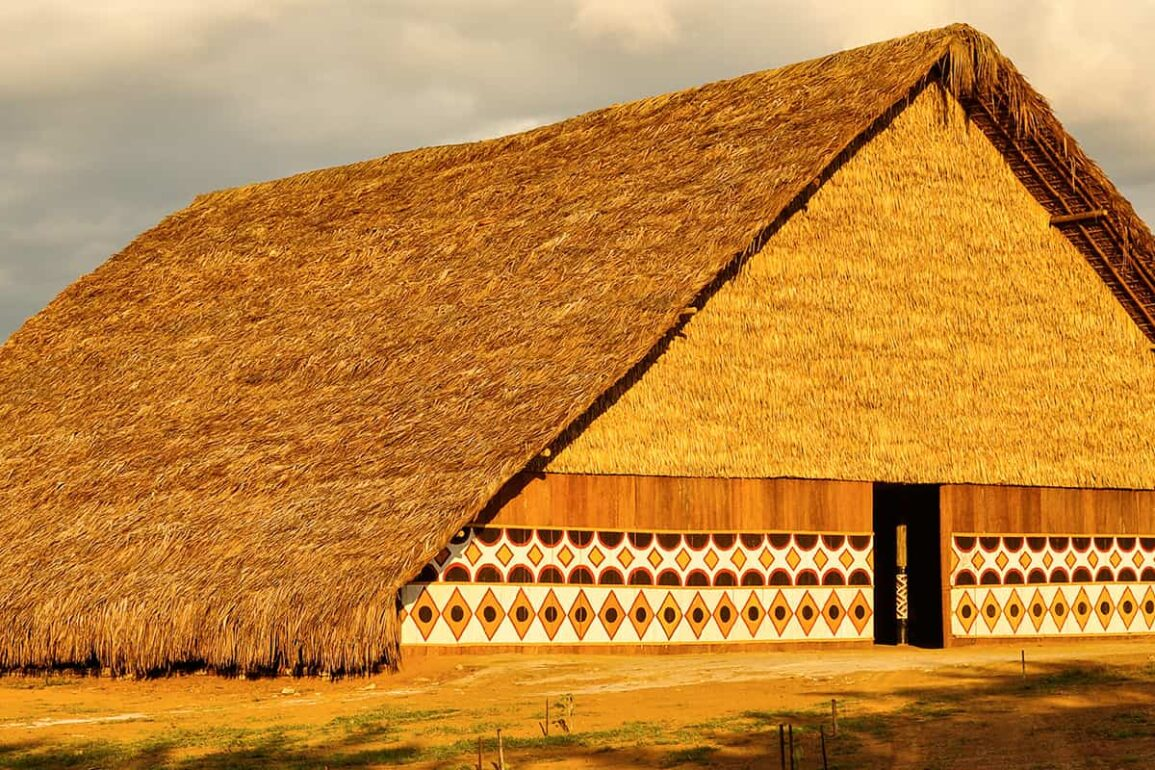
\includegraphics[width=.8\linewidth]{./IMG/revistaSIM_Arquitetura-Indigena_Destaque_Credito-Julio-Duarte_Shutterstock.com_-1155x770.jpg}
\end{center}


\vfill
\pagebreak

\begin{center}
	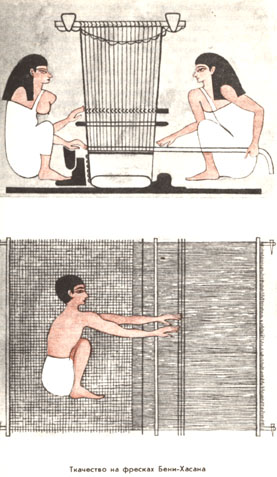
\includegraphics[height=.9\textheight]{./IMG/tear-egito.jpg}
\end{center}

\null
\columnbreak

\begin{center}
	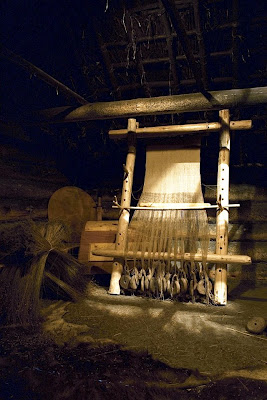
\includegraphics[height=.9\textheight]{./IMG/tear-europa.jpg}
\end{center}

\null
\columnbreak

\begin{center}
	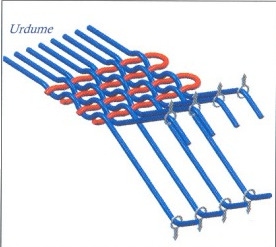
\includegraphics[width=.9\linewidth]{./IMG/Tecer.jpg}
\end{center}

\null
\columnbreak

\begin{center}
	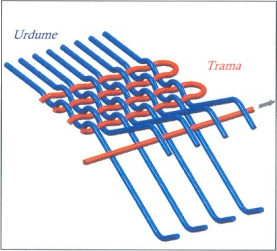
\includegraphics[width=.9\linewidth]{./IMG/Tecer2.jpg}
\end{center}

\end{multicols}
\vfill
\pagebreak


